\section{Method}
\label{sec:method}

% Explain how you approached the stated problem. Aim to be detailed enough for others to reproduce your results. If necessary, refer to your code.

The method chapter presents the approach to the stated problem, and aims to give details for complete replicability. However, for full details, the implementation can be found on GitHub\footnote{https://github.com/jakeberggren/TDDE16-Text-Mining-Project/tree/main}. The method is divided into three distinct parts, which will all be described in the subsequent subsections. 

\subsection{Loading and pre-preprocessing data}
\label{subsec:method-data}

First, train and test data was loaded into separate pandas DataFrames, using the python package pandas\footnote{https://pandas.pydata.org}. As explained in section \ref{sec:data}, 50\% of the test data was first removed due to API constraints in the later methods (see section \ref{subsec:method-llm-approach}). The original data was labeled using numbers, and not the names of each condition, which is why one of the first steps was to translate each number into the corresponding labels. Correct translation was provided by the data set authors in conjunction with the data. Next, the data was explored by both looking at the structure (in terms of class count and balance), and creating word clouds for each class to get a better sense of common words, both across the classes, but also words that signify each class. Figure \ref{fig:word-clouds} shows the result of these word-clouds.

\begin{figure}[ht]
    \centering
    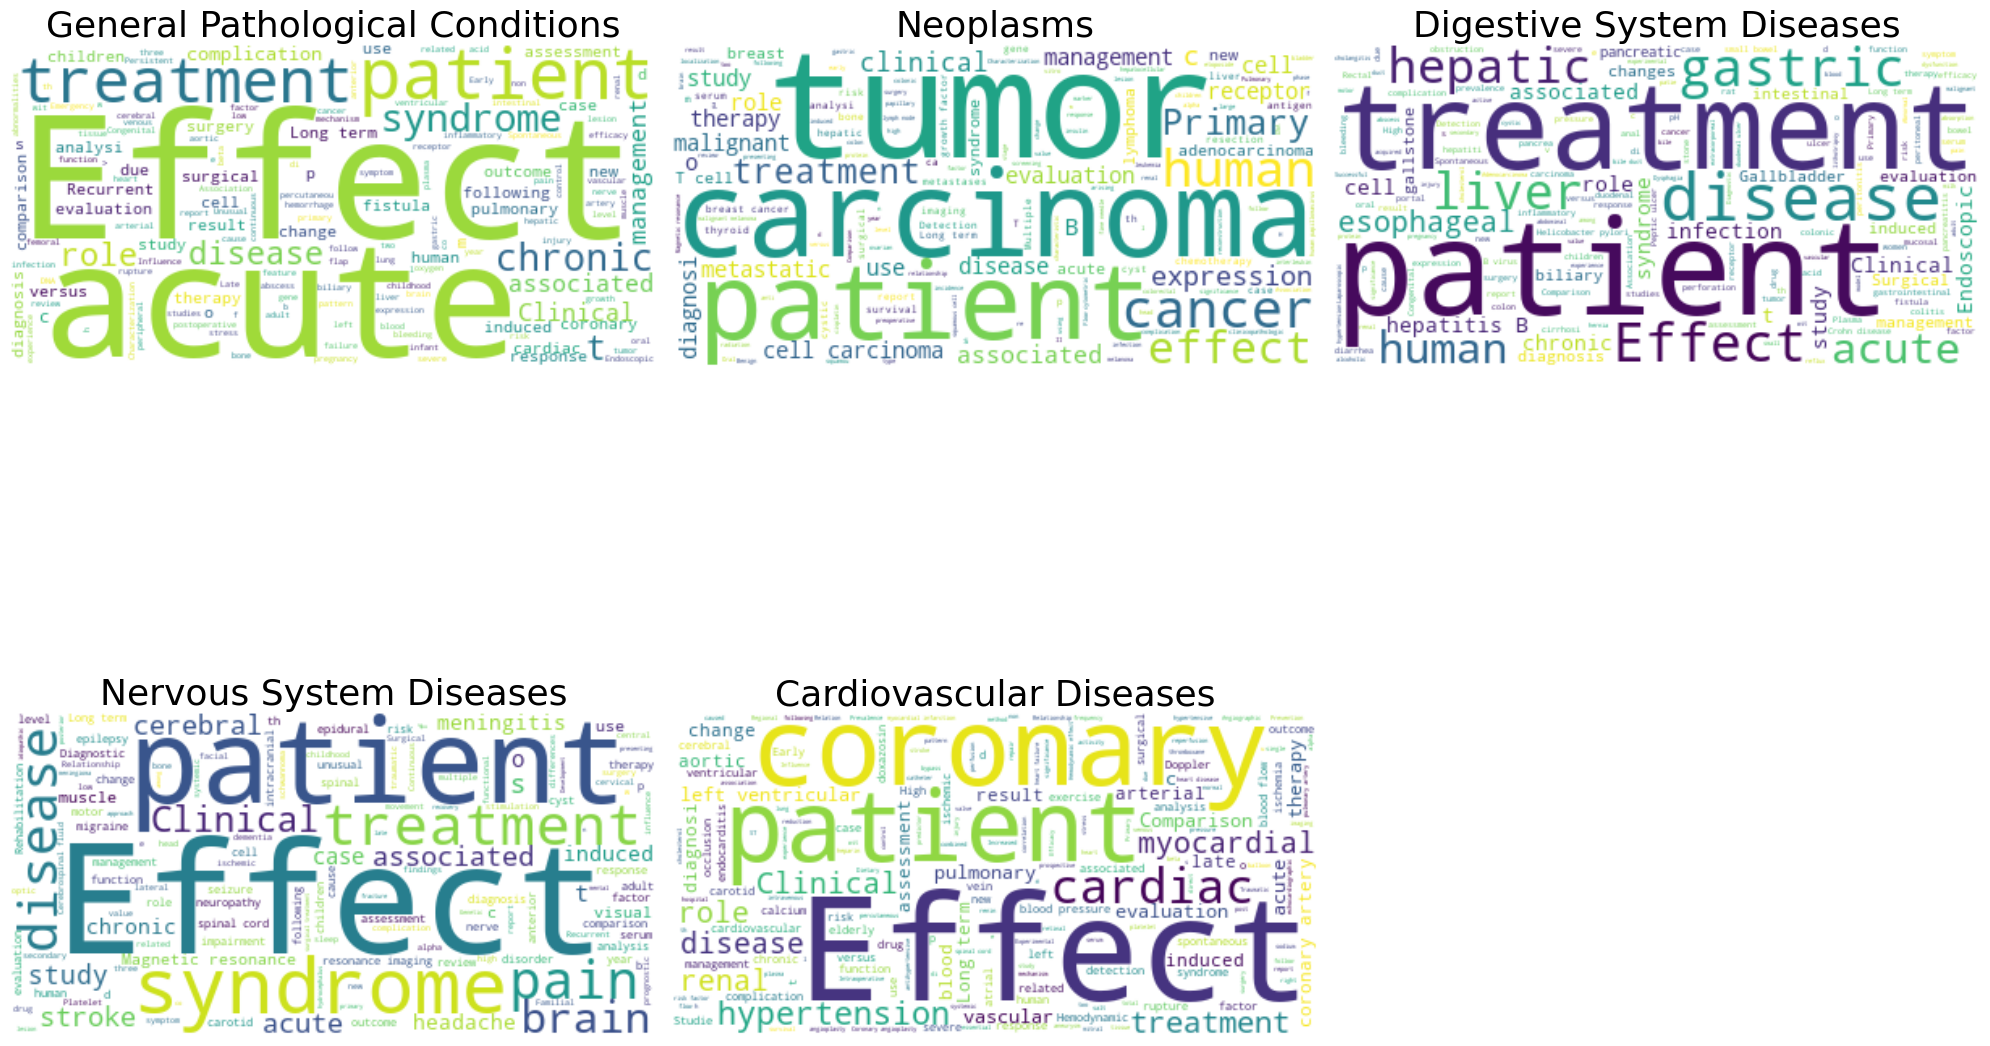
\includegraphics[width=\columnwidth]{report/figures/word-clouds.png}
    \caption{Word clouds showcasing common words in each class.}
    \label{fig:word-clouds}
\end{figure}

The data exploration resulted in two main insights. First, the training data was quite imbalanced, which resulted in additional pre-processing by undersampling to the minority class, as explained in section \ref{sec:data}. Second, insights from the word-clouds resulted in the experimenting with medical stop-word removal to test if this could increase the performance of the statistical approach, which is further explained in subsection \ref{subsec:method-statistical-approach}.

\subsection{Statistical approach}
\label{subsec:method-statistical-approach}

The statistical approach to the problem implements four different techniques, all common in multi-class classification tasks: 1. Multinomial Naive Bayes, 2. Support Vector Machines (with linear kernel), 3. Random Forest, and 4. Gradient Boosting. These techniques were all implemented using count vectorization, meaning that the training documents are transformed into document-term matrices representing the frequency of each token in each document. Initially, no stop-word removal was applied.

Each technique was then fitted using the undersampled training data, and later tested on the test data. Metrics accuracy, precision, recall and f1-score were then computed by comparing predicted labels to the gold label in the test data. Results were saved into .csv files, and later visualized as confusion matrices and a bar plot for each metric and technique. The implementation was largely done using built-in packages from scikit-learn as well as visualized using Matplotlib\footnote{https://matplotlib.org/stable/} and Seaborn\footnote{https://seaborn.pydata.org/\#}, two common statistical data visualization tools.

Following the analysis of the word clouds seen in figure \ref{fig:word-clouds}, it was concluded that experimentation with stop-word removal could possibly increase the performance of the statistical approach. Some clear trends from the analysis could be seen. For example, \textit{general pathological conditions} contain words like “chronic” and “acute” (also found in other categories but less frequently). \textit{Neoplasms} include the words “tumor”, “cancer”, and “carcinoma”. \textit{Digestive System Diseases} include “gastric” and “hepatic”, and \textit{Cardiovascular Diseases} include “cardiac”. many of these are of course not surprising. However, some words are quite common across all the categories, such as “patient”, “effect” and “treatment”.

Stop-word removal was done in three different ways. First, common English stop-words were removed using Natural Language Toolkit, or NLTK\footnote{https://www.nltk.org} a python package commonly used for statistical NLP. Second, clinical stop-words were removed by adding stop-words used by Ganesan et al. in their work on discovering related clinical concepts using large amounts of clinical notes \cite{Ganesan2016DiscoveringNotes}. The full stop-words list can be found on the authors' GitHub.\footnote{https://github.com/kavgan/clinical-concepts}. Third, three additional stop-words were manually added due to their frequency and lack of meaning in the context of medical abstracts: “patient”, “effect”, and “treatment”. Finally, any duplicates were removed from the stop-words list.

Previous experiments were then re-done, this time removing stop-words as explained above. Further, Results were computed, saved and visualized in the same way as previously explained.

\subsection{LLM approach}
\label{subsec:method-llm-approach}

The LLM approach, similar to the statistical approach, implements four different techniques separated into four experiments respectively: 1. Zero-shot classifier, 2. One-shot classifier, 3. Few-shot classifier, and 4. Similarity based classifier, all further explained in further detail in the subsequent subsections. Similarly to the statistical approach, results from each experiment were collected and computed in the form of accuracy, precision, recall and f1-score by comparing to the test data gold label. The results were then aggregated and visualized in the same way as in the statistical approach, in order for easy comparisons between the different approaches.

All four LLM approaches makes use of the OpenAI API for access to the model GPT-3.5 Turbo\footnote{https://platform.openai.com/docs/models/gpt-3-5-turbo}. While not the latest model from OpenAI, GPT-3.5 Turbo is more cost-effective, while still offering very high complexity. For the similarity based classifier, OpenAI's embedding model was used\footnote{https://platform.openai.com/docs/models/embeddings}. Further, the python package LangChain\footnote{https://www.langchain.com} was employed to simplify the implementation for all techniques presented.

\subsubsection{Zero-shot classifier}

For the Zero-shot classifier, a simple zero-shot prompt was created, which can be seen in figure \ref{code:zero-shot-prompt_template}.

\begin{Verbatim}[frame=single, framesep=3mm, framerule=0.5pt, rulecolor=\color{black}]
template = """Classify the given 
medical abstract into one of these
5 medical conditions:

1. neoplasms
2. digestive system diseases
3. nervous system diseases
4. cardiovascular diseases
5. general pathological conditions

Medical abstract: {abstract}
Condition: """
\end{Verbatim}
\vspace{-1.5em}
\captionsetup{type=figure}
\caption{Zero-shot prompt template. \{abstract\} acts as a placeholder for the actual medical abstract to classify.}
\label{code:zero-shot-prompt_template}
\vspace{1em}

Each medical abstract in the test set was then classified using GPT-3.5 Turbo and the prompt template in figure \ref{code:zero-shot-prompt_template}. The output data from the model was post processed to only include the actual prediction (in the case that the model produced more surrounding words other than one of the 5 medical conditions). Further, in cases where no prediction was made by the model, one of the 5 medical conditions were chosen at random.

\subsubsection{One-shot classifier}

The One-shot classifier was implemented in a similar manner. First, \textit{one} example from each category was sampled from the training data at random. Next, the previous prompt was built upon, adding the following parts as shown in figure \ref{code:one-shot-prompt_template}:

\begin{Verbatim}[frame=single, framesep=3mm, framerule=0.5pt, rulecolor=\color{black}]
.
.
4. cardiovascular diseases
5. general pathological conditions

Base your answer on the following 
examples of medical abstracts and 
correctly labeled conditions:

Medical abstract: {example_abstract}
Condition: {example_condition}

Medical Abstract: {abstract}
Condition:""""
\end{Verbatim}
\vspace{-1.5em}
\captionsetup{type=figure}
\caption{One- and few-shot prompt template.}
\label{code:one-shot-prompt_template}
\vspace{1em}

Post-processing was made in the same way as previously explained. 

\subsubsection{Few-shot classifier}

Using the same prompt as for the one-shot classifier, shown in figure \ref{code:one-shot-prompt_template}, the few-shot classifier was implemented by including \textit{three} examples (instead of one) of each category of medical abstracts from the training data to the model. No other changes were made to the implementation or prompt.

\subsubsection{Similarity based classifier}

The similarity based classifier was implemented with inspiration from Schopf et al. \cite{Schopf2022EvaluatingApproaches}, which proposed the original dataset used in this study. The method is based on comparing training data embeddings to the embedded input abstract, assigning it the same condition label as the most similar example from the training data. This is done by embedding the training data using the embedding model provided by OpenAI, and then storing the embeddings in a Chroma DB\footnote{https://www.trychroma.com} vector database. Each example in the test data is then subsequently embedded and similarity matched to the training data in the vector database by cosine distance, and assigned to the label with the lowest similarity score (lower is better, or "more similar").